\documentclass[12pt]{article}

\usepackage{graphicx}
\graphicspath{{../Fichier_Image}}
\title{Hypothèse 3.(c) Porte Bureaux Regulation}
\author{Thibault Clodion}

\begin{document}

\maketitle % Permet d'afficher le titre, l'author etc

\underline{Hypothèse :} Certain bureaux (même grand) doivent avoir qu'une seule porte pour réguler les flux
\newline\newline
\underline{Expérience :}Des simulations avec le bâtiment en photo, une où il a une porte (comme sur la photo) et une où il y en a deux dont une à gauche, donc il y aura plus de régulation des flux
\newline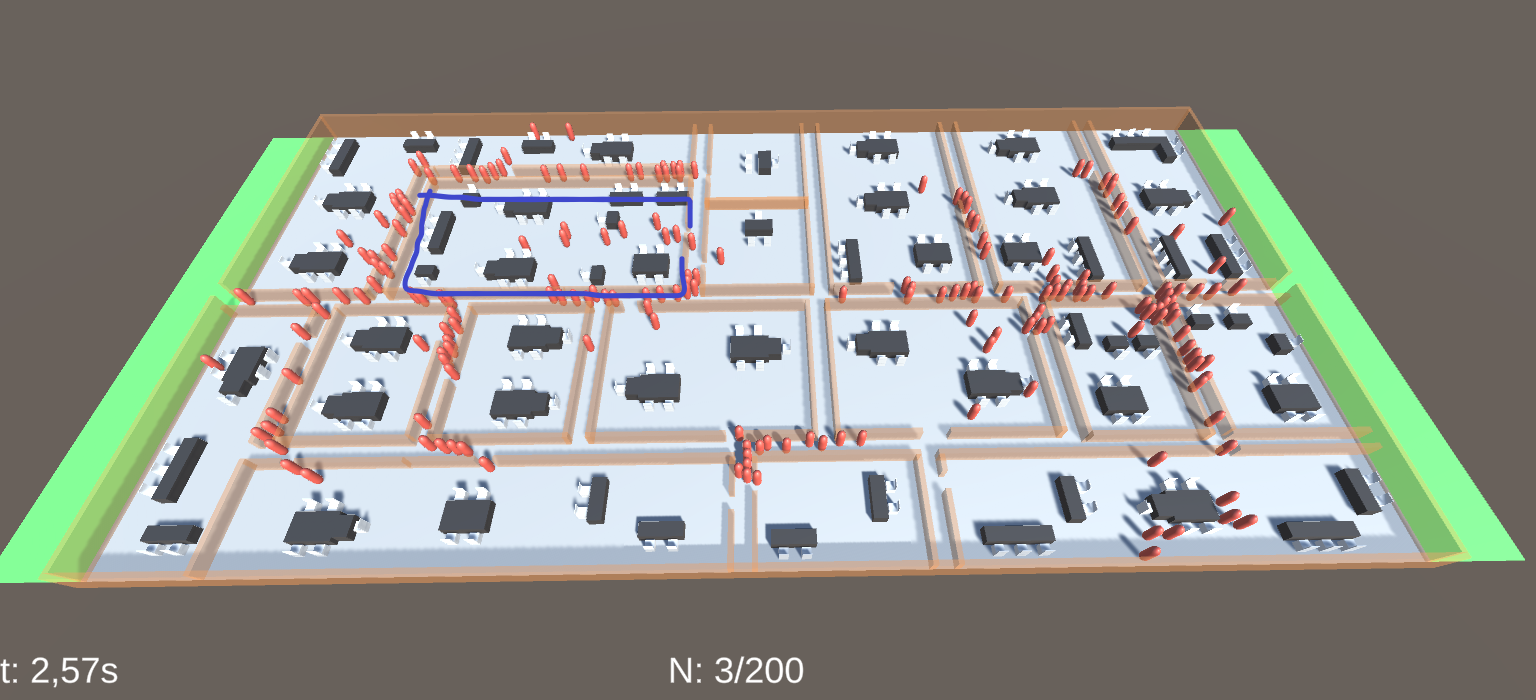
\includegraphics[scale=0.17]{7. bureau 1 porte.png}\newline
\newline
(peut-être le temps qu'ils fassent le tour revient à diviser le flux à voir.)
\newline\newline


\end{document}